In the framework of advanced, active hand prosthetics, nowadays we are
witnessing a sort of technology transfer from robotics and
mechatronics. Touch Bionics's i-LIMB \cite{ilimb} prosthetic hand,
with its five degrees-of-freedom, is a real breakthrough with respect
to the previous state-of-the-art, Otto Bock's SensorHand Speed
\cite{sensorhand}, which is essentially an open-close
mechanism. Dexterity of hand prostheses is still far from that of
state-of-the-art non-prosthetic mechanical hands, such as, e.g., the
DLR II \cite{Hua2006} (not to mention a human hand, of course), but
things are getting better thanks to the aforementioned
inter-disciplinary exchange (see Figure \ref{fig:hands}). Several
EU-funded projects (e.g., CyberHand \cite{CyberHand} and SmartHand
\cite{smarthand}) testify the enthusiasm in the field.

\begin{figure}
  \begin{tabular}{ccc}
    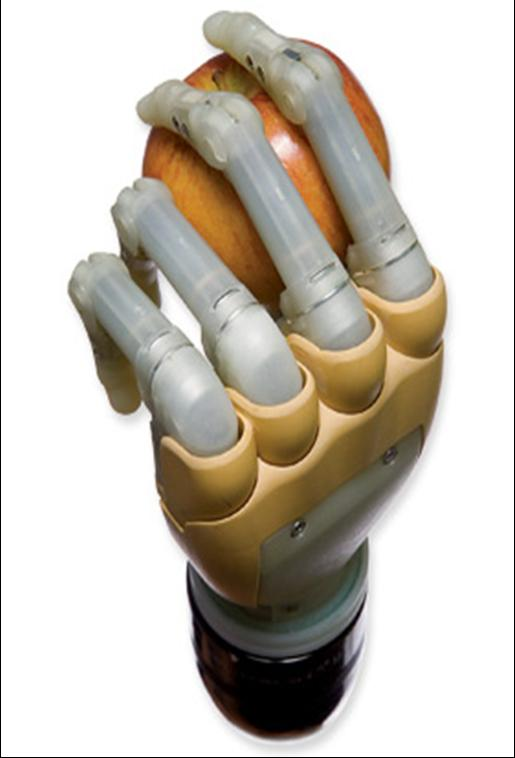
\includegraphics[width=0.14\textwidth]{figs/hands_TB.jpg} &
    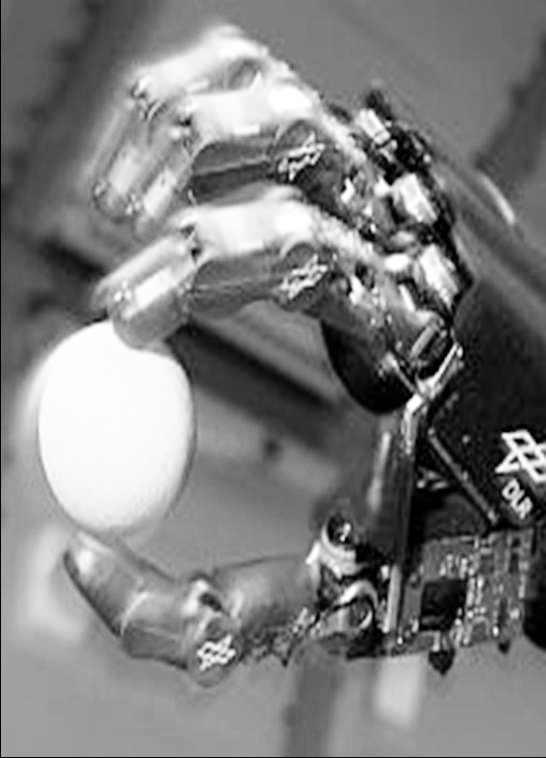
\includegraphics[width=0.14\textwidth]{figs/hands_DLRII.jpg} &
    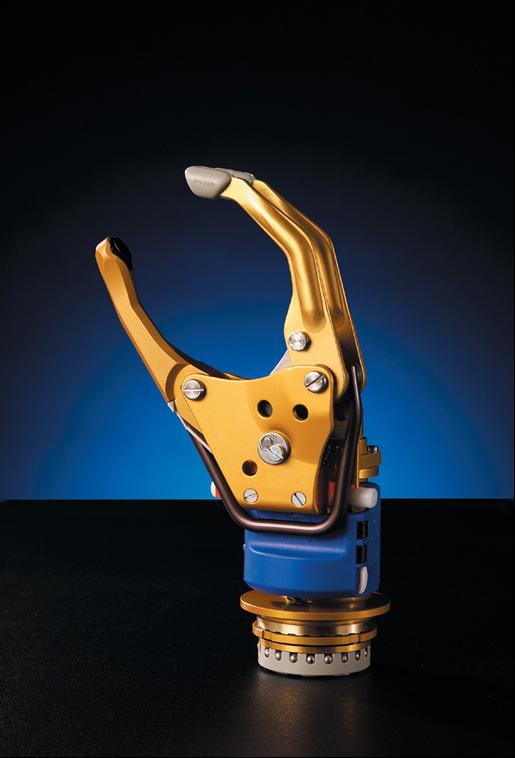
\includegraphics[width=0.14\textwidth]{figs/hands_OB.jpg} \\
    $(a)$ & $(b)$ & $(c)$
  \end{tabular}
  \caption{$(a)$ Touch Bionics's i-LIMB prosthetic hand (reproduced
    from \cite{ilimb}); $(b)$ the DLR-II mechanical hand; $(c)$ Otto
    Bock's SensorHand Speed (reproduced from \cite{sensorhand}).}
  \label{fig:hands}
\end{figure}

The most used technique for interfacing the patient with the
prosthesis is surface electromyography (sEMG). It works by detecting
the activation potentials of the patient's stump residual muscles, and
it is widely employed in the commercial setting; it is relatively
cheap and totally non-invasive. But the control schema employed so far
is rather poor, using two or three electrodes to issue an
``open/close'' command or, in the more advanced case of the i-LIMB, to
choose among a predefined set of grasp shapes. The electrodes are
associated with large muscles in the patient's stump, such as, e.g.,
the wrist flexor and extensor. The result is a highly non-natural form
of control (for instance, wrist flexion corresponding to opening) and
there is no chance of controlling the desired force.

All in all, a general sense of frustration impends, as far as control
is concerned. How is an amputee supposed to \emph{naturally} command
the prosthesis what to do (i.e., how to grasp an object) and with what
force? Recent research to this end has shown that excellent results
can be obtained by using \emph{machine learning} techniques such as,
e.g., Support Vector Machines (SVM), to let the prosthesis itself
\emph{adapt to the patient}, rather than the other way round. The idea
is that, as it has been shown in, e.g.,
\cite{smagt,dunlop,2008.ICRA,2008.BioCyb,Sebelius2005}, such a system
can be trained to recognize EMG patterns of the patient's stump
muscles, which are then mapped to hand positions and/or a force
exerted by the prosthesis. This way the mechanical hand can be driven
with a degree of finesse unknown so far; and as well, its force can be
controlled, which is possibly even more important. A final very
agreeable point is that standard, commercially available EMG
electrodes can be used to this end.

The idea is that of improving the patient's quality of life by
providing an \emph{adaptive prosthesis}, so that he/she enters a
virtuous loop of \emph{reciprocal learning}, whereas so far the
patient has to learn how to control the prosthesis from scratch. To
this aim, that is, to shorten the patient's training time, we believe it is
desirable to \emph{pre-train} the prosthesis with a model which will
be then refined and then adapted on-line, little by little; this, as
opposed to shipping an ``empty'' prosthesis which has to be trained
from scratch.

In machine learning, this is called \emph{model adaptation}: a system
which adapts to a new data distribution, as this distribution shifts
with time. Here we envision the application of this framework to a
model trained on pre-existing patients, which would then serve as a
basic model for new patients; we claim that adapting such pre-loaded
models to a new patient would lead to a quicker and better training,
rather than training from scratch. We address the problem like this:
\textbf{FRANCESCO...}

To corroborate our claim, we apply this idea to a large set of EMG
data collected from $10$ healthy subjects. During the experiments 
we asked to the subject to grasp a force sensor in different 
conditions and using three different grips; meanwhile, we  
recorded the electrical activity of the muscles that mostly are
involved in the hand / wrist movements and the force exerted by 
the subject on a off-the-shelf medical load cell. Then we estimated
from the acquired data a raw \emph{control signal} by computing the
RMS of the EMG signals \textbf{AND...SVM}.

The experimental results
show that our intuition is correct, to the point that
\textbf{FRANCESCO: riassunto dei risultati}.

The paper is structured as follows: Section \ref{sec:mms} shows how
the EMG database was collected; Section \ref{sec:math} gives
mathematical details about our method; Section \ref{sec:exp} shows the
experimental results, and lastly Section \ref{sec:concl} contains the
conclusions.
